
\begin{frame}[c]
  \frametitle{Case V : Waste Form Degradation Rate and Inventory}
These runs varied the waste form degradation rate and the waste inventory mass 
factor.  There were forty runs corresponding to eight values of the waste form degradation 
rate and five values of the mass factor.

\begin{table}[ht!]
\centering
\footnotesize{
\begin{tabular}{|l|l|l|r|r|}
\multicolumn{5}{c}{\textbf{Simulation Cases}}\\
\hline
\textbf{Case} & \textbf{Parameter} & \textbf{Units} & \textbf{Min. Value} & \textbf{Max. Value}\\
\hline
V     & $R_{WFDeg.}$           & $[yr^{-1}]$       & $10^{-9}$    &  $10^{-2}$ \\
      & Inventory              & [MTHM]         & $10^{-4}$    &  $10^1$ \\
\hline
\end{tabular}
\caption{Each dual and single parameter simulation case had 40 simulation 
groups of 100 realizations each.}
\label{tab:Cases}
}
\end{table}


\end{frame}

\begin{frame}[c]
  \frametitle{Case V : Waste Form Degradation Rate and Inventory}

Safety indicators for post closure repository performance have been developed by 
the \gls{UFD} campaign which utilize the inventory multiplier that was varied in 
this study \cite{nutt_generic_2009}. These indicators are normalized by a 
normalization factor (100 mrem/yr) recommended by the \gls{IAEA} as the limit to 
``relevant critical members of the public'' \cite{iaea_international_1996}. The functional form for 
this safety indicator for a single waste category, \gls{HLW}, is just 

\begin{align}
SI_{G} &= \left(\frac{\sum_{i=1}^{N}D_{G,i}(I_i, F_{d})}{100mrem/yr}\right)[GWe/yr].
\label{indicator}
\intertext{where}
SI_{G} &= \mbox{Safety indicator for disposal in media type G}[GWe/yr]\nonumber\\
N &= \mbox{Number of key radionuclides considered in this indicator}\nonumber\\
D_{G,i} &= \mbox{Peak dose rate from isotope i in media type G}[mrem/yr]\nonumber\\
F_{d} &= \mbox{Fractional waste form degradation rate}[1/yr].\nonumber
\end{align}
\end{frame}

\begin{frame}[c]
  \frametitle{Case V : Waste Form Degradation Rate and Inventory}
\begin{figure}[ht!]
\centering
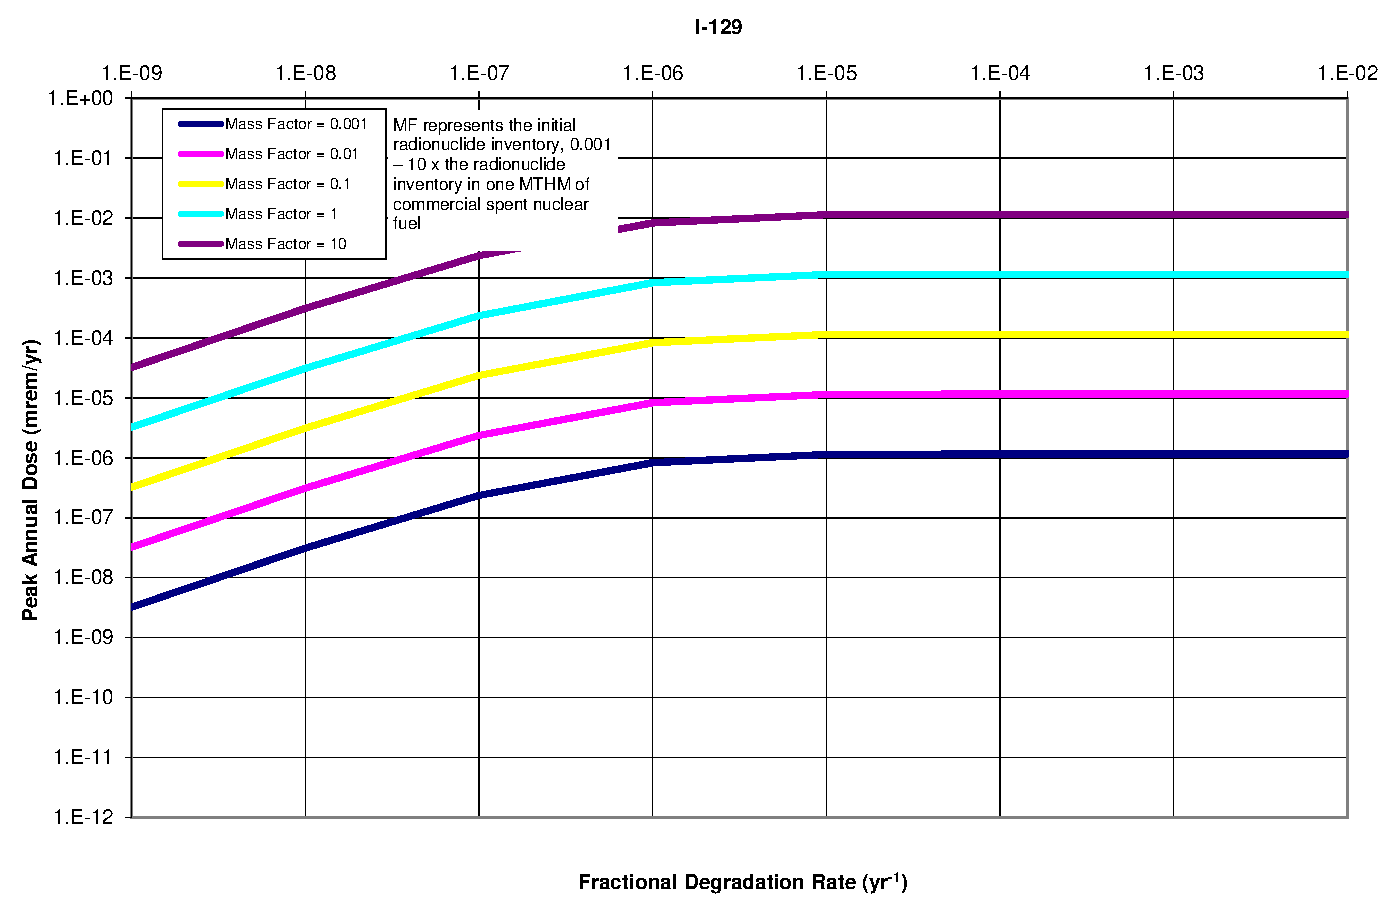
\includegraphics[width=0.8\textwidth]{WFDegAndInv/I-129.eps}
\caption{
Highly soluble and non-sorbing $^{129}I$ demonstrates a direct proportionality between dose rate and 
fractional degradation rate until a turnover where other natural system 
parameters dampen transport.} 
\label{fig:WFDegI129}
\end{figure}
\end{frame}

\begin{frame}[c]
  \frametitle{Case V : Waste Form Degradation Rate and Inventory}

\begin{figure}[ht!]
\centering
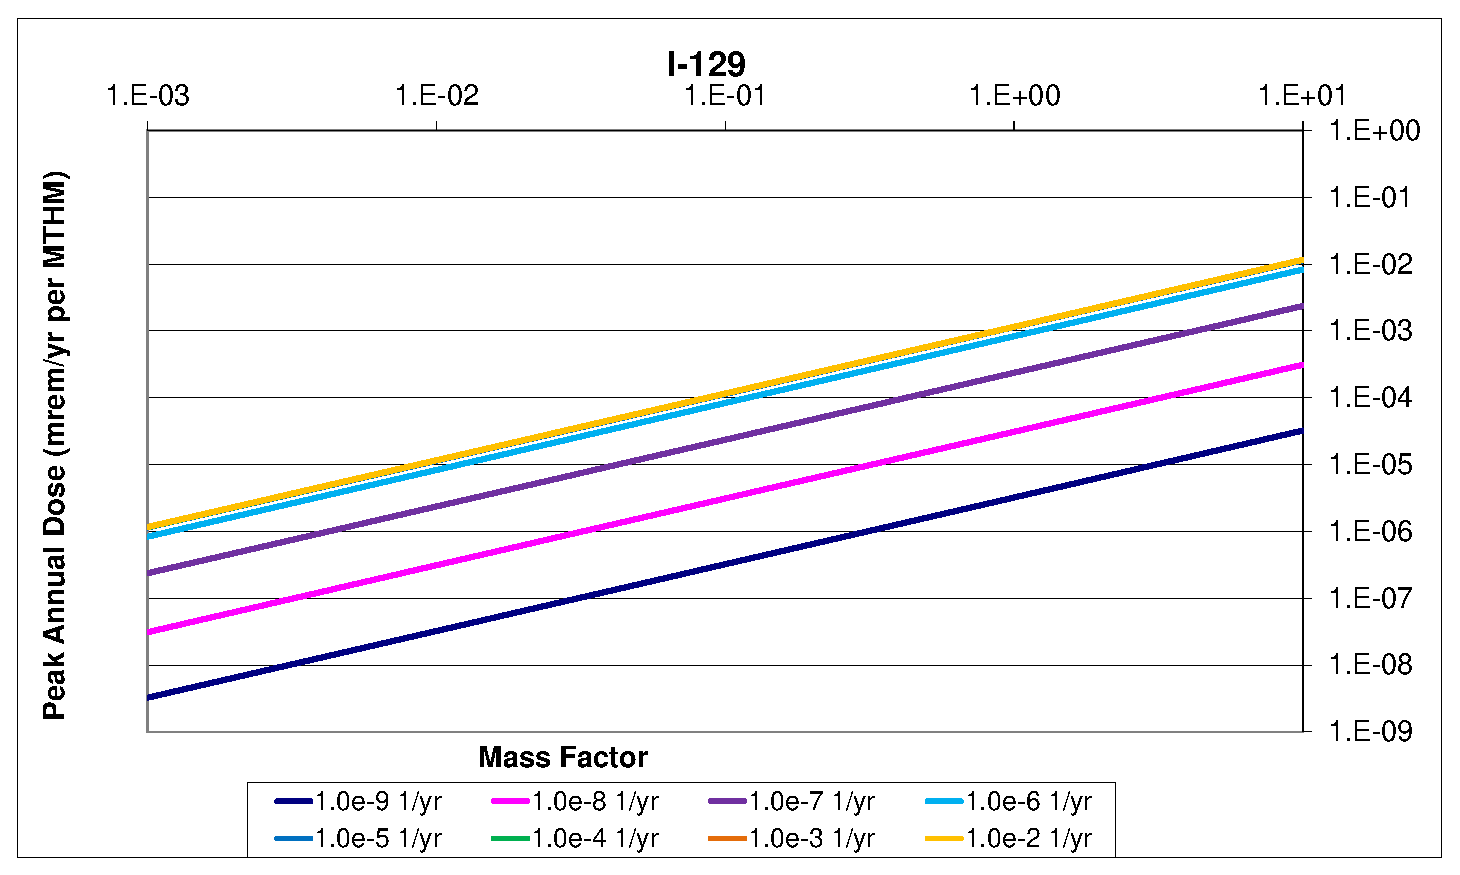
\includegraphics[width=0.8\textwidth]{WFDegAndInv/I-129-MF.eps}
\caption{
Highly soluble and non-sorbing $^{129}I$ domonstrates a direct 
proportionality to the inventory multiplier.}
\label{fig:WFDegI129MF}
\end{figure}
\end{frame}

\begin{frame}[c]
  \frametitle{Case V : Waste Form Degradation Rate and Inventory}

\begin{figure}[ht!]
\centering
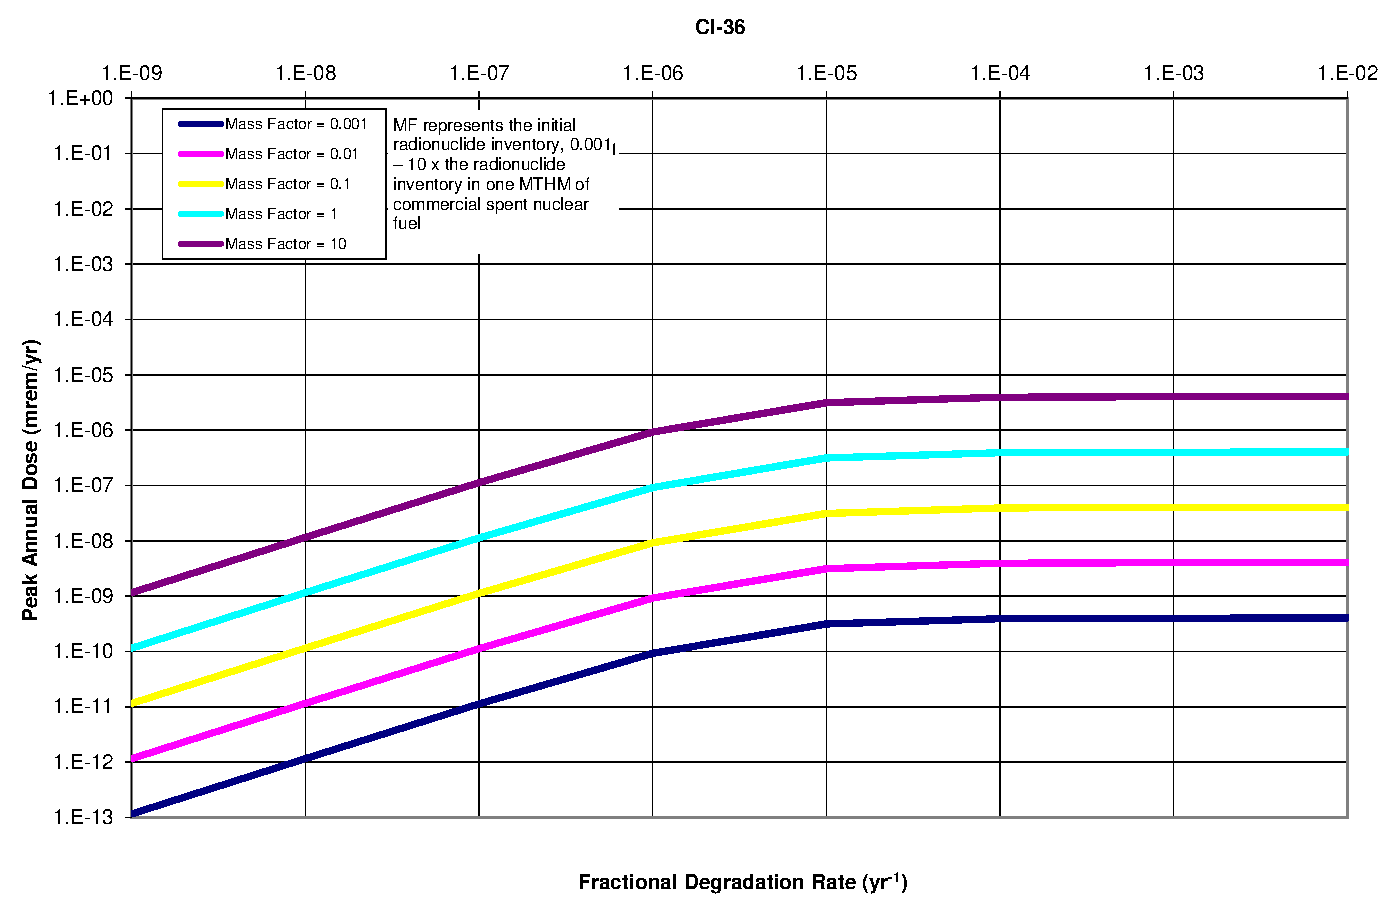
\includegraphics[width=0.8\textwidth]{WFDegAndInv/Cl-36.eps}
\caption{
Highly soluble and non-sorbing $^{36}Cl$ demonstrates a direct proportionality between dose rate and 
fractional degradation rate until a turnover where other natural system 
parameters dampen transport.} 
\label{fig:WFDegCl36}
\end{figure}

\end{frame}

\begin{frame}[c]
  \frametitle{Case V : Waste Form Degradation Rate and Inventory}
\begin{figure}[ht!]
\centering
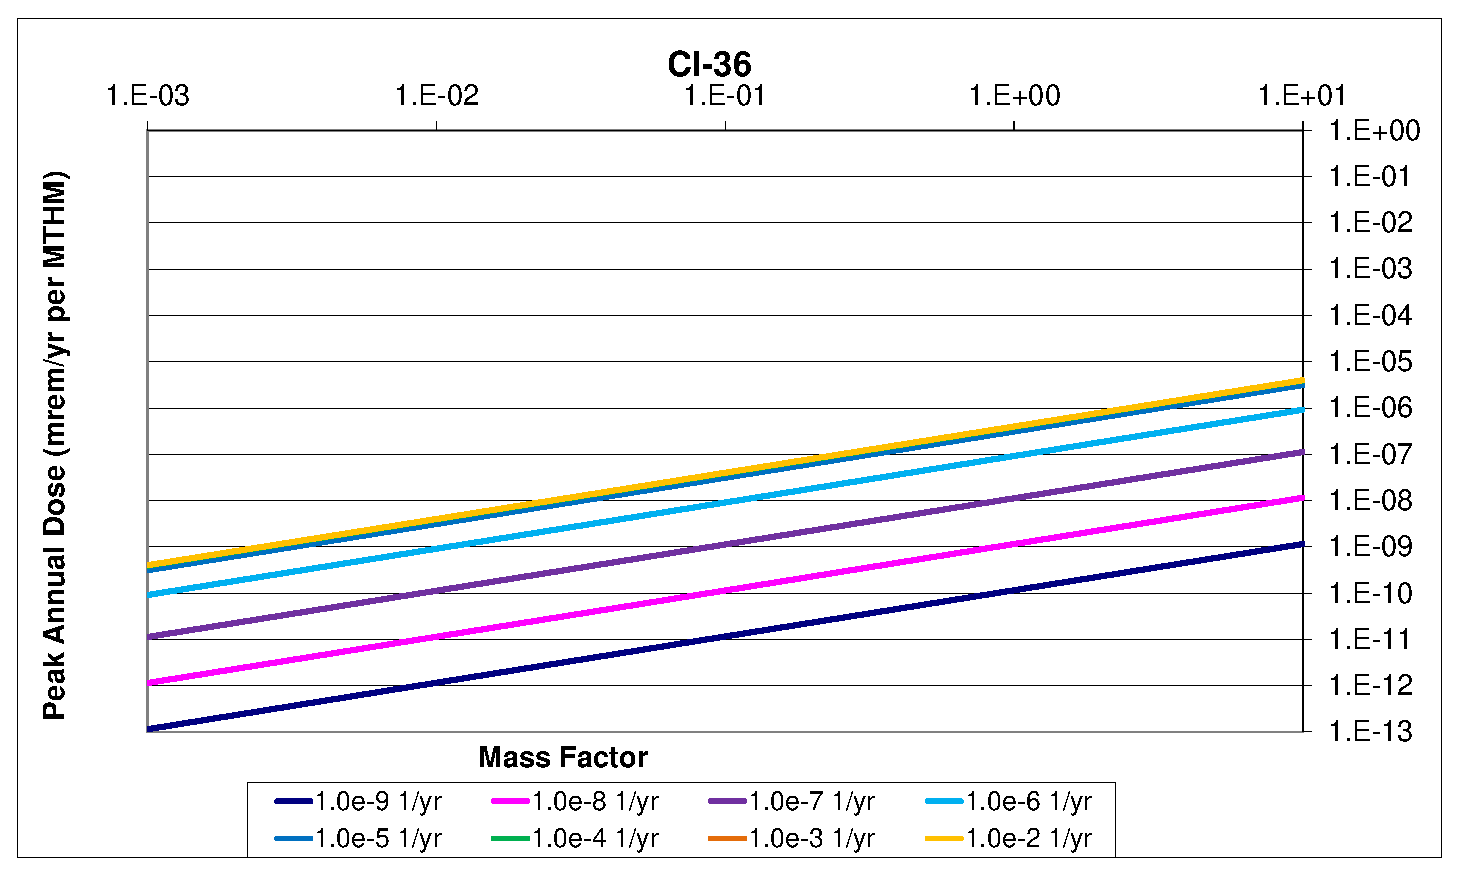
\includegraphics[width=0.8\textwidth]{WFDegAndInv/Cl-36-MF.eps}
\caption{
Highly soluble and non-sorbing $^{129}I$ domonstrates a direct 
proportionality to the inventory multiplier.}
\label{fig:WFDegCl36MF}
\end{figure}
\end{frame}

\begin{frame}[c]
  \frametitle{Case V : Waste Form Degradation Rate and Inventory}
The peaks for solubility limited, sorbing elements such as $Tc$ and $Np$, on the 
other hand, have a more dramatic turnover.  For very high degradation rates, the 
dependence on mass factor starts to round off due to attenuation by solubility 
limits.


\begin{figure}[ht!]
\centering
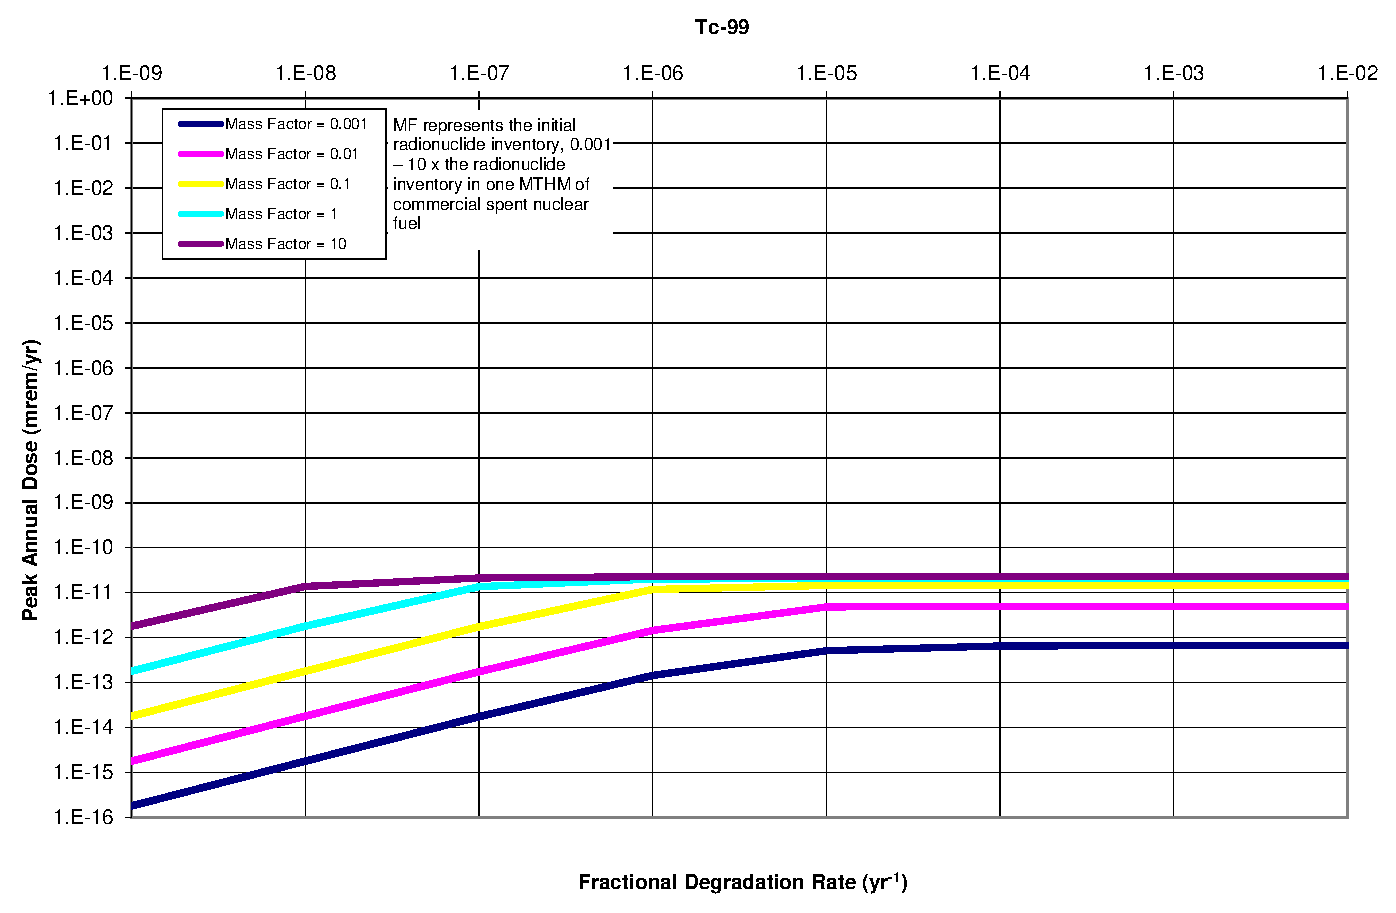
\includegraphics[width=0.8\textwidth]{WFDegAndInv/Tc-99.eps}
\caption{
Solubility limited and sorbing $^{99}Tc$ demonstrates a direct proportionality 
to fractional degradation rate until attuation by its solubility limit and other 
natural system parameters. } 
\label{fig:WFDegTc99}
\end{figure}
\end{frame}

\begin{frame}[c]
  \frametitle{Case V : Waste Form Degradation Rate and Inventory}

\begin{figure}[ht!]
\centering
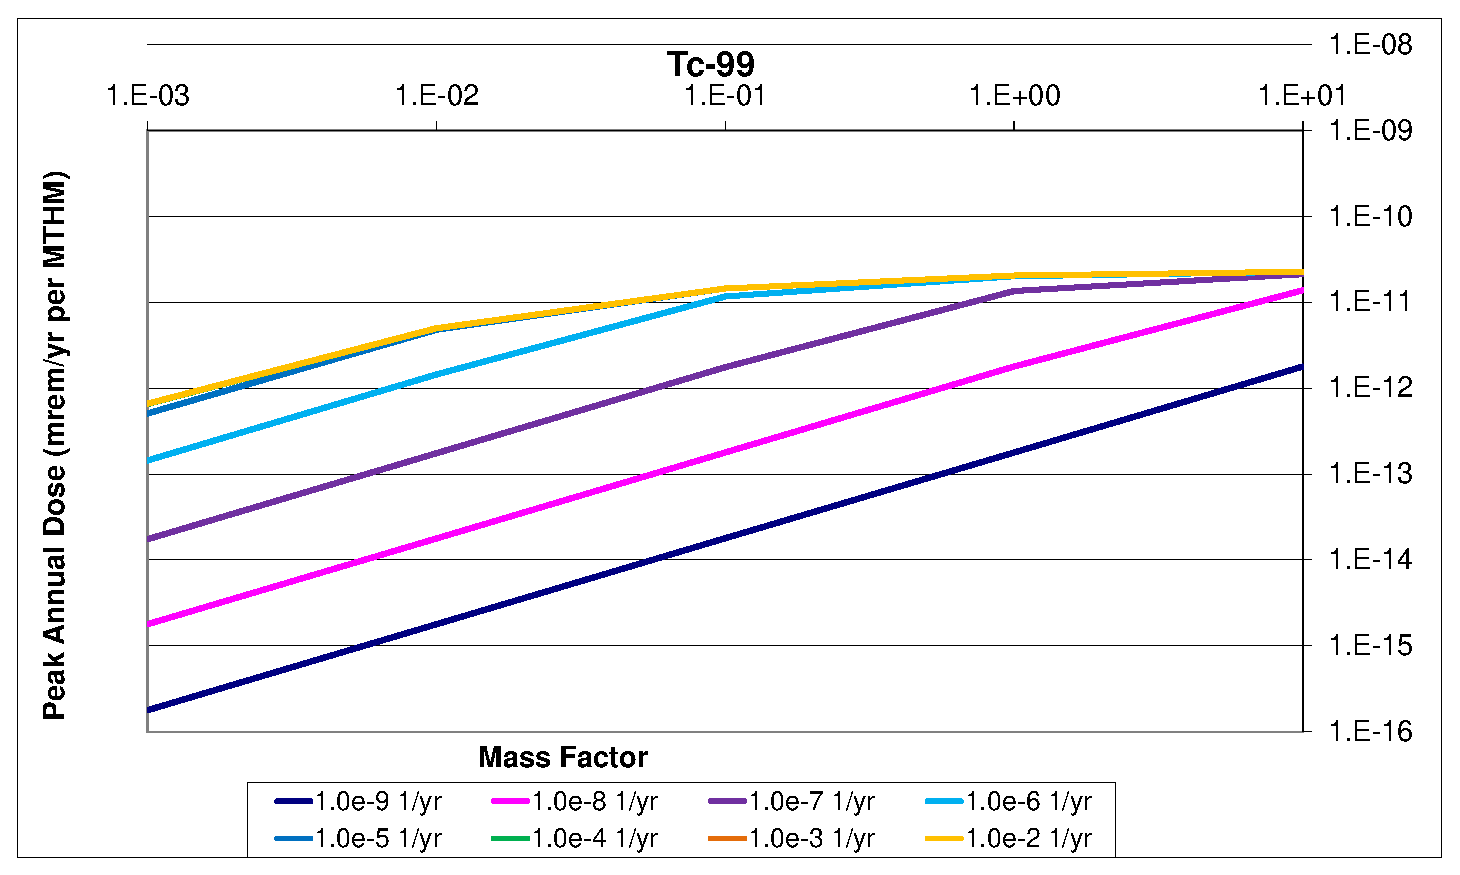
\includegraphics[width=0.8\textwidth]{WFDegAndInv/Tc-99-MF.eps}
\caption{
  Solubility limited and sorbing $^{99}Tc$ demonstrates a direct proportionality 
to fractional degradation rate until attuation by its solubility limit and other 
natural system parameters. } 
\label{fig:WFDegTc99MF}
\end{figure}

\end{frame}

\begin{frame}[c]
  \frametitle{Case V : Waste Form Degradation Rate and Inventory}

\begin{figure}[ht!]
\centering
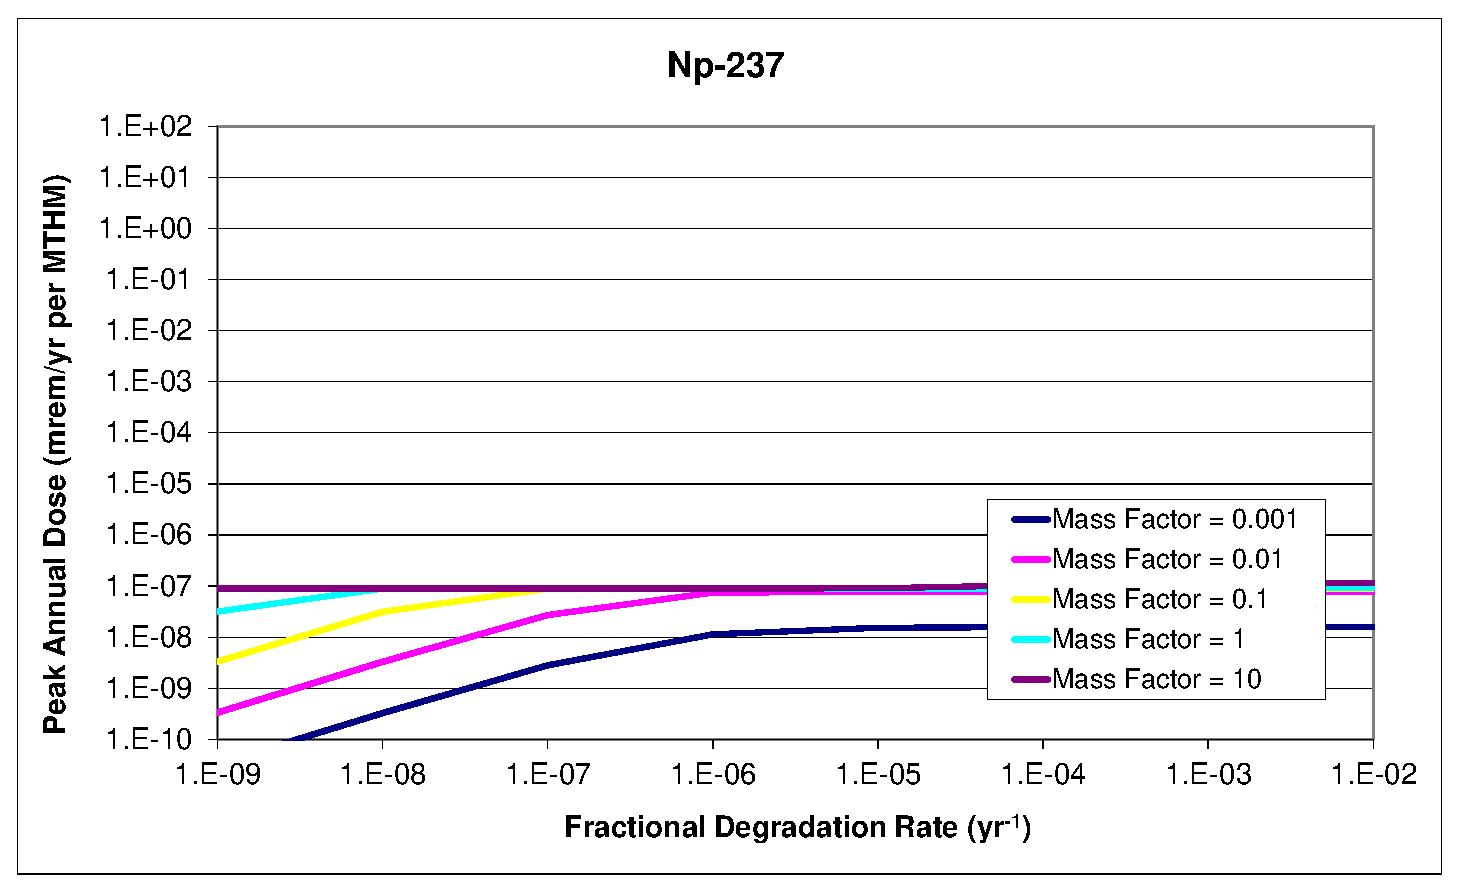
\includegraphics[width=0.8\textwidth]{WFDegAndInv/Np-237.eps}
\caption{
  Solubility limited and sorbing $^{237}Np$ demonstrates a direct proportionality 
to fractional degradation rate until attuation by its solubility limit and other 
natural system parameters. } 
\label{fig:WFDegNp237}
\end{figure}
\end{frame}

\begin{frame}[c]
  \frametitle{Case V : Waste Form Degradation Rate and Inventory}

\begin{figure}[ht!]
\centering
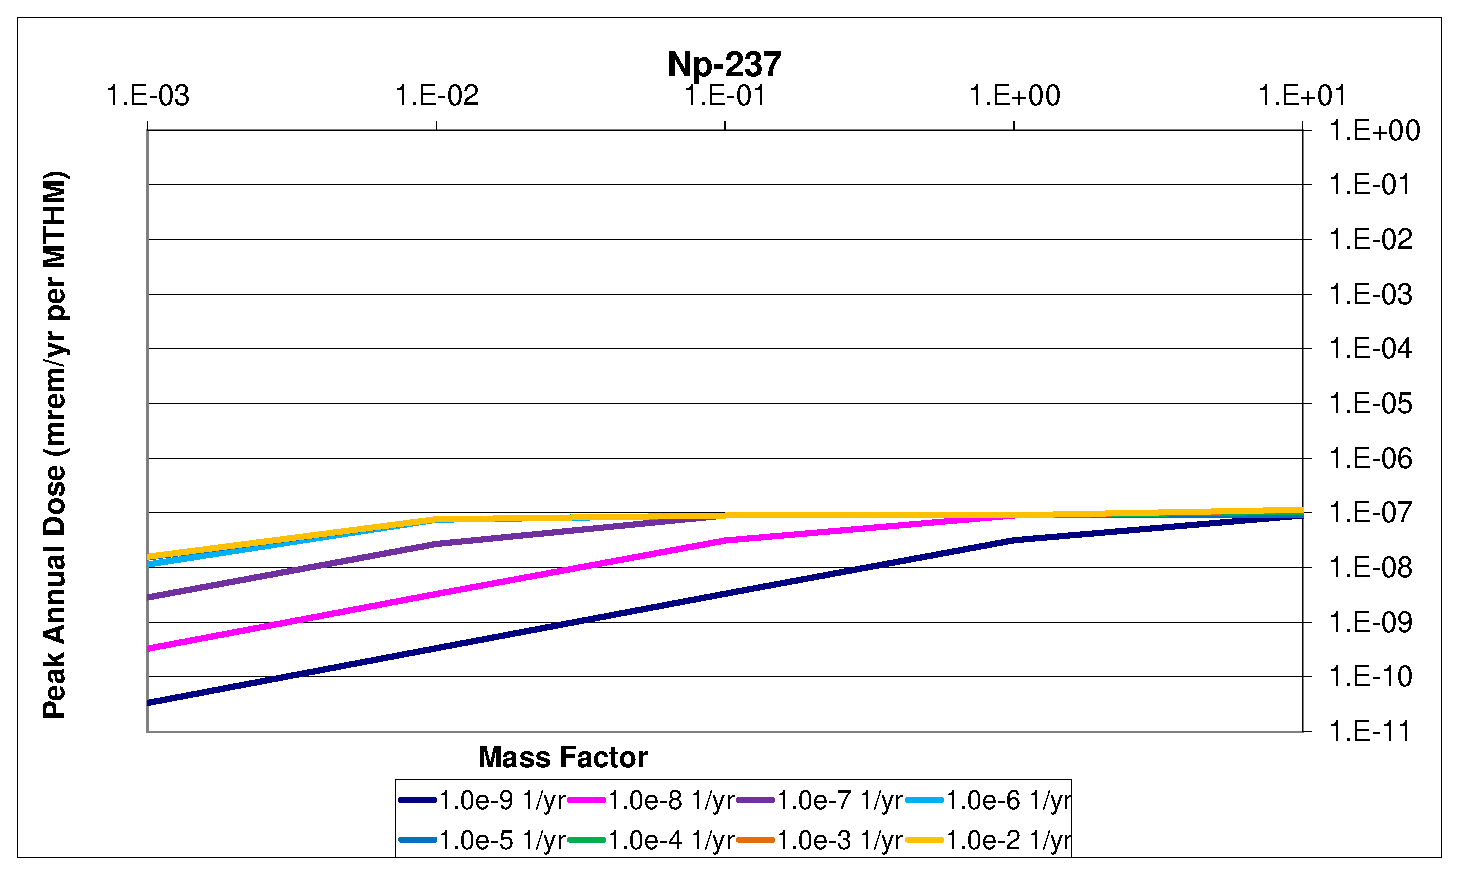
\includegraphics[width=0.8\textwidth]{WFDegAndInv/Np-237-MF.eps}
\caption{
  Solubility limited and sorbing $^{237}Np$ demonstrates a direct proportionality 
to fractional degradation rate until attuation by its solubility limit and other 
natural system parameters. } 
\label{fig:WFDegNp237MF}
\end{figure}

\end{frame}

